\documentclass{butexFR}
\usepackage{tabularray}
\usepackage{subcaption}     % subfigure / subtable



\titre{Développement efficace}
\UE{Algorithmie}
\sujet{SAÉ 3.02 - Labyrinthe}
\enseignant{Mme Everaere}
\eleves{Victor Bredelle \\ Antonin Marouze \\ Romain Harlaut \\ Angèl Zheng \\ Baptiste Lavogiez}


\begin{document}

\fairepagedegarde
\fairemarges
\tabledematieres

\section{Introduction}
Ce rapport présente la partie algorithmique du projet \textbf{SAÉ S3.02 - Labyrinthe}, une application permettant la génération de labyrinthes variés.

L'objectif est de décrire notre solution et d'en démontrer la pertinence au regard de l'efficacité d’exécution et des exigences du sujet.

\section{Investissement dans le projet}
\textbf{Groupe G3.3}

\begin{itemize}
\item Victor Bredelle
\item Antonin Marouze
\item Romain Harlaut
\item Angèl Zheng
\item Baptiste Lavogiez 
\end{itemize}

\begin{table}[h]
\centering
\begin{tblr}{
colspec = {ccccccc},
hlines, vlines,
row{1} = {bg=gray!20},
column{1}= {bg=gray!40}
}
Nom & Victor & Antonin & Romain & Angèl & Baptiste & Total \\
Part & 60\% & 0\% & 0\% & 10\% & 30\% & 100\% \\
\end{tblr}
\caption{Répartition de l'investissement}
\label{tab:repartition}
\end{table}

\tsec{Victor}

\begin{itemize}
    \item Algorithme du jalon 1.
    \item Algorithme parfait version TP (jalon 2).
    \item Algorithme de fusion initial (matrice d'entiers).
\end{itemize}

\tsec{Antonin}

\tsec{Romain}

\tsec{Angèl}

\begin{itemize}
    \item Algorithme de déplacement de monstre.
\end{itemize}

\tsec{Baptiste}

\begin{itemize}
\item Algorithme distance entrée/sortie (Jalon 2).
\item Algorithme pour les labyrinthes aléatoires (Jalon 2).
\item Benchmarks de performance des labyrinthes et modélisation.
\item Algorithme de fusion optimisé (union-find).
\end{itemize}

\tsecnonum{Le groupe}

Chaque section est écrite par la personne l'ayant réalisée, et éventuellement relue par le groupe.

\newpage

\section{Structures de données pour les labyrinthes}

\subsection{Labyrinthes parfaits}

Les labyrinthes parfaits sont représentés à l’aide de deux structures de données simples et efficaces :

\begin{enumerate}
\item Un tableau de booléens représentant les murs verticaux, de taille [largeur-1][hauteur] ;
\item Un tableau de booléens représentant les murs horizontaux, de taille [hauteur-1][largeur].
\end{enumerate}

Les positions sont représentées par une structure \texttt{Position}, étant un simple couple \textit{x et y}.

Cette représentation, identique à celle utilisée dans le TP sur les labyrinthes parfaits, constitue la structure minimale pour modéliser correctement un labyrinthe. Elle se limite à des variables primitives, garantissant une excellente compacité mémoire et une absence totale de redondance.

Ces deux tableaux permettent un accès en temps constant aux murs, ce qui les rend parfaitement adaptés aux différents algorithmes de génération (parcours en profondeur, fusion / Union-Find, suppression aléatoire de murs).

Nous n’avons pas proposé de structure alternative : la structure du TP est déjà très satisfaisante en termes de simplicité, de rapidité d’accès et de coût mémoire, et se révèle tout aussi efficace pour les labyrinthes aléatoires, qui héritent directement de cette représentation.

\subsection{Labyrinthes aléatoires}
Puisque les labyrinthes aléatoires héritent des labyrinthes parfaits dans notre cas, leur structure est identique.

\subsection{Implémentation}

Classe : \texttt{fr.univlille.labyrinth.model.maze.Maze}

Attributs : \texttt{boolean[][] horizontalWalls}, \texttt{boolean[][] verticalWalls}

Méthodes d'accès : \texttt{isWall(int y1, int x1, int y2, int x2)}

Lien : \href{https://gitlab.univ-lille.fr/sae302/2025/G2_SAE3.3/-/tree/master/labyrinth/src/main/java/fr/univlille/labyrinth/model/maze?ref_type=heads}{Package \texttt{maze}}

\newpage

\section{Algorithmes de génération}

Toutes les implémentations \textbf{d'algorithme} sont trouvables dans le package \texttt{algorithm} : \href{https://gitlab.univ-lille.fr/sae302/2025/G2_SAE3.3/-/tree/master/labyrinth/src/main/java/fr/univlille/labyrinth/model/algorithm?ref_type=heads}{Package \texttt{algorithm}}

L'implémentation précise de chaque algorithme est indiquée dans les sous-sections suivantes.

\info{Dans la suite, nous appellerons \texttt{PERFECT} l'algorithme de génération par parcours en profondeur (DFS) utilisé dans le TP2, et \texttt{FUSION} l'algorithme de génération par fusion d'ensembles basé sur une structure Union-Find.}

\subsection{Distance entrée/sortie}

\textbf{Cet algorithme sera utilisé dans les algorithmes à venir.}

Le placement d’une distance entrée/sortie est ici traité comme un algorithme à part entière. Le respect strict de la distance nécessite en effet de réaliser, depuis l’entrée, un parcours maîtrisé vers la sortie en contrôlant précisément la distance qui les sépare.

\subsubsection{Algorithme utilisé}

Une approche par niveaux sera utilisée ici. L'algorithme sera un \textbf{parcours en largeur}.

\newpage

\subsubsection{Pseudo-code}

On note :
\begin{itemize}
\item \( d \) : la distance cible entre l'entrée et la sortie.
\end{itemize}

\begin{codeboxlang}{pseudocode}
// Etape 1 : Initialisation
creer une position aleatoire entree dans le labyrinthe
creer une file vide
creer une map distances vide
creer une liste positionsResultat vide
ajouter entree a la file
ajouter (entree, 0) a distances
niveauActuel = 0
distanceReelle = 0

// Etape 2 : Parcours en largeur par niveaux
tant que la file n'est pas vide :
    tailleNiveau = taille de la file

    // Arret si on depasse la distance cible
    si niveauActuel > d :
        arreter le parcours

    // Si on atteint exactement la distance cible
    si niveauActuel = d :
        pour i de 0 a tailleNiveau :
            position = retirer premier element de la file
            ajouter position a positionsResultat
            distanceReelle = niveauActuel
            arreter le parcours

    // Explorer le niveau actuel
    pour i de 0 a tailleNiveau :
        positionCourante = retirer premier element de la file
        pour chaque direction {haut, bas, gauche, droite} :
            prochaine = calculer position adjacente selon direction
            si prochaine valide et prochaine non visitee et pas de mur :
                ajouter (prochaine, niveauActuel + 1) a distances
                ajouter prochaine a la file

    distanceReelle = niveauActuel
    niveauActuel = niveauActuel + 1

// Etape 3 : Si distance impossible, prendre le maximum
si positionsResultat est vide :
    pour chaque (position, distance) dans distances :
        si distance = distanceReelle :
            ajouter position a positionsResultat

// Etape 4 : Placer entree et sortie
sortie = choisir aleatoirement une position dans positionsResultat
definir entree dans le labyrinthe
definir sortie dans le labyrinthe
mettre a jour la distance effective avec distanceReelle
\end{codeboxlang}

Notre solution permet alors un strict respect de la distance entrée/sortie, et surtout, un calcul de la distance maximale possible afin de ramener la distance voulue à celle maximale si celle voulue était impossible dans ce labyrinthe. Cette notion est \textbf{importante pour la suite}.

La mise à jour de la distance effective permet, entre autres, d’informer la structure de labyrinthe que la distance souhaitée a changé, afin d’offrir un retour explicite à l’utilisateur.

\subsubsection{Structures de données utilisées}

Pendant l'exécution, l'algorithme utilise principalement une file et un dictionnaire.

Quant au retour, l'algorithme utilise un objet \texttt{distanceResultat} contenant :
  
\begin{itemize}
\item Une liste de positions.
\item La distance effective.
\end{itemize}

Puis, la liaison (prochaine sous-section) choisit aléatoirement une position parmi la liste.
La distance effective est ensuite attribuée au labyrinthe, afin d'avertir de l'impossibilité de réaliser celle initialement voulue.

\subsubsection{Pertinence}

\begin{itemize}
\item La file est indispensable puisqu'il s'agit d'un parcours en largeur. Elle nous permet d'explorer plusieurs niveaux à la fois.
\item Le dictionnaire sert à associer une position à sa distance, permettant de vérifier rapidement si une position a déjà été visitée et de récupérer les positions à la distance cible.
\end{itemize}

L'objet \texttt{distanceResultat} permet une transmission facilitée des résultats vers les autres classes.

Enfin, la motivation principale quant au choix des structures est l'efficacité. La structure choisie dans ce cas est minimale et comporte uniquement ce dont nous avons besoin pour déterminer une position aléatoire respectant la distance demandée (ou maximum si impossible).

\subsubsection{Implémentation}

Classe : \texttt{fr.univlille.labyrinth.model.algorithm.pathsearch.MazeDistance}

Méthode principale : \texttt{calculateAllDistances(Maze maze, Position start, int targetDistance)}

\href{https://gitlab.univ-lille.fr/sae302/2025/G2_SAE3.3/-/blob/master/labyrinth/src/main/java/fr/univlille/labyrinth/model/algorithm/pathsearch/MazeDistance.java?ref_type=heads}{\texttt{MazeDistance}}

\newpage 

\subsection{Liaison distance/algorithme}

\textbf{Cette sous-section ne présente pas un algorithme en particulier, mais décrit le fonctionnement commun à l’ensemble, afin de rendre les explications plus claires.}

Tous les algorithmes de génération héritent de l'abstraction \texttt{MazeAlgorithm}, qui applique toujours le même schéma :

\begin{enumerate}
    \item \textbf{Génération de la structure} : création des murs selon l’algorithme choisi (PERFECT, FUSION ou RANDOM)
    \item \textbf{Placement de l’entrée et de la sortie} : application de l’algorithme de distance pour respecter la distance demandée
\end{enumerate}

Cela permet de réunir les comportements communs ainsi que de bénéfier d'une modularité accrue des algorithmes.

\subsubsection{Pseudo-code}

\begin{codeboxlang}{pseudocode}
fonction genererLabyrintheComplet(labyrinthe, distanceCible):

    // Étape 1 : génération de la structure
    pour chaque mur du labyrinthe:
        mettre le mur à présent
    appliquerAlgorithmeDeGeneration(labyrinthe)
        // PerfectAlgorithm, FusionKruskalUnion ou RandomAlgorithm

    // Étape 2 : placement de l'entrée et de la sortie
    entree = choisirPositionAleatoire(labyrinthe)
    resultat = calculerDistancesAvecContrainte(labyrinthe, entree, distanceCible)
    sortie = choisirAleatoirement(resultat.positionsValides)

    fixerEntreeDuLabyrinthe(labyrinthe, entree)
    fixerSortieDuLabyrinthe(labyrinthe, sortie)
    enregistrerDistanceEntreeSortie(labyrinthe, resultat.distanceReelle)
\end{codeboxlang}


\subsubsection{Architecture}

La méthode abstraite \texttt{generateMaze()} est spécifique à chaque algorithme, tandis que \texttt{generateExitAndPlayer()} est commune : elle garantit pour tous les labyrinthes la même gestion de la distance entrée/sortie, tout en facilitant l’ajout de nouveaux algorithmes.

\subsubsection{Implémentation}

Classe principale : \texttt{fr.univlille.labyrinth.model.algorithm.MazeAlgorithm}

Méthodes :
\begin{itemize}
    \item \texttt{generateMaze(Maze maze)} : implémentée dans chaque algorithme
    \item \texttt{generateExitAndPlayer(Maze maze)} : placement commun entrée/sortie
\end{itemize}

\href{https://gitlab.univ-lille.fr/sae302/2025/G2_SAE3.3/-/blob/master/labyrinth/src/main/java/fr/univlille/labyrinth/model/algorithm/MazeAlgorithm.java?ref_type=heads}{MazeAlgorithm}

\newpage 

\subsection{Labyrinthes parfaits : Version TP}

\subsubsection{Algorithme utilisé}

L’algorithme utilisé est celui du parcours en profondeur. L’objectif est de placer des murs partout dans le labyrinthe, puis de le parcourir en supprimant les murs gênants au passage. Cela garantit que le résultat sera un labyrinthe parfait.

\newpage

\subsubsection{Pseudo-code}

\begin{codeboxlang}{pseudocode}
// Etape 1 : Initialisation
creer une position aleatoire comme entree dans le labyrinthe
creer une pile vide de positions
creer un tableau de booleens "visitee" initialise a faux
ajouter l'entree a la pile
marquer l'entree comme visitee

// Etape 2 : Parcours en profondeur
tant que la pile n'est pas vide :
    positionCourante = sommet de la pile
    directions = [haut, bas, gauche, droite]
    melanger l'ordre des directions aleatoirement
    positionTrouvee = faux

    // Explorer les directions possibles
    pour chaque direction dans directions :
        nouvellePosition = positionCourante + direction
        si nouvellePosition est dans le labyrinthe et non visitee :
            marquer nouvellePosition comme visitee
            ajouter nouvellePosition a la pile
            supprimer le mur entre positionCourante et nouvellePosition
            positionTrouvee = vrai
            arreter la boucle des directions

    // Si aucune direction valide, retour arriere
    si positionTrouvee = faux :
        retirer positionCourante de la pile
\end{codeboxlang}

\subsubsection{Structures de données utilisées}

Pendant l'exécution, l'algorithme utilise principalement :

\begin{itemize}
    \item une \textbf{pile} de positions pour le parcours en profondeur ;
    \item un \textbf{tableau de booléens} \texttt{visitée} indiquant si une cellule a déjà été explorée.
\end{itemize}

La représentation du labyrinthe (murs horizontaux et verticaux) reste celle décrite en Section~3 et n'est pas modifiée ici.


\subsubsection{Pertinence}

La pile est essentielle pour le parcours en profondeur, permettant de revenir en arrière lorsque nécessaire. Le tableau de booléens permet de suivre les cellules déjà visitées, évitant ainsi les cycles et garantissant que chaque cellule est visitée une seule fois.

\subsubsection{Implémentation}

Classe : \texttt{fr.univlille.labyrinth.model.algorithm.PerfectAlgorithm}

Méthodes principales : \texttt{generateMaze(Maze maze)}, \texttt{algoProfondeur(int height, int width)}

\href{https://gitlab.univ-lille.fr/sae302/2025/G2_SAE3.3/-/blob/master/labyrinth/src/main/java/fr/univlille/labyrinth/model/algorithm/PerfectAlgorithm.java?ref_type=heads}{Lien vers l'implémentation}

\newpage 

\subsection{Labyrinthes parfaits : Version originale - Fusion}

\subsubsection{Algorithme utilisé}

L'algorithme utilisé est celui de la fusion aléatoire. Son objectif est d'attribuer un numéro différent à chaque case. Tant que toutes les cases n'ont pas le même numéro, on choisit deux cases adjacentes et on fusionne leurs numéros. Cela génère un labyrinthe parfait, mais avec une apparence différente, généralement jugée meilleure de celle obtenue par le parcours en profondeur.

Cet algorithme repose sur le principe des ensembles disjoints. Initialement, chaque cellule du labyrinthe forme son propre ensemble. L'algorithme fusionne progressivement ces ensembles en supprimant les murs entre cellules adjacentes appartenant à des ensembles différents, jusqu'à ce qu'il ne reste qu'un seul ensemble connexe.

Nous avons implémenté deux versions de cet algorithme :
\begin{enumerate}
    \item Une version initiale utilisant une matrice d'entiers ;
    \item Une version optimisée utilisant la structure Union-Find.
\end{enumerate}

\newpage

\subsubsection{Pseudo-code - Version initiale}

\begin{codeboxlang}{pseudocode}
// Etape 1 : Initialisation - generer une grille de numeros differents
generer une grille ou chaque cellule a un numero unique

// Etape 2 : Fusion progressive des ensembles
tant que la grille contient au moins deux numeros differents :
    position = choisir une position aleatoire
    direction = choisir une direction aleatoire
    positionVoisine = position + direction

    // Fusionner si les deux cellules ont des numeros differents
    si positionVoisine est dans le labyrinthe et que les numeros de position et positionVoisine sont differents :
        supprimer le mur entre position et positionVoisine
        fusionner les cellules : toutes les cases ayant le numero de positionVoisine
            prennent le numero de position

\end{codeboxlang}

\subsubsection{Pseudo-code - Version optimisée (Union-Find)}

Cette version optimisée utilise la structure de données Union-Find pour éviter de parcourir toute la grille à chaque fusion.

On note :
\begin{itemize}
\item \( parent[i] \) : le parent du noeud i dans la structure Union-Find ;
\item \( size[i] \) : la taille de l'ensemble contenant i ;
\item \( components \) : le nombre de composantes connexes restantes.
\end{itemize}

\begin{codeboxlang}{pseudocode}
// Etape 1 : Initialisation de la structure Union-Find
total = hauteur * largeur
creer parent[total] où parent[i] = i pour tout i
creer taille[total] où taille[i] = 1 pour tout i
composantes = total

// Fonction de recherche avec compression de chemin
fonction find(x):
    si parent[x] != x:
        parent[x] = find(parent[x])  // compression de chemin
    retourner parent[x]

// Fonction d'union par taille
fonction union(a, b):
    pa = find(a)
    pb = find(b)
    si pa = pb: retourner

    // Attacher le plus petit arbre au plus grand
    si taille[pa] < taille[pb]:
        parent[pa] = pb
        taille[pb] += taille[pa]
    sinon:
        parent[pb] = pa
        taille[pa] += taille[pb]

    composantes = composantes - 1

// Etape 2 : Fusion progressive jusqu'a obtenir un seul ensemble
tant que composantes > 1:
    direction = direction aleatoire
    position = position aleatoire dans le labyrinthe
    positionVoisine = position + direction

    si positionVoisine est valide:
        id1 = index de position
        id2 = index de positionVoisine

        // Fusionner si dans des ensembles differents
        si find(id1) != find(id2):
            supprimer le mur entre position et positionVoisine
            union(id1, id2)
\end{codeboxlang}

\subsubsection{Structures de données utilisées}

\textbf{Version initiale (matrice d'entiers) :}

La première version utilisait une matrice d'entiers \texttt{grid[hauteur][largeur]} où chaque cellule contenait son numéro d'ensemble. À chaque fusion entre deux ensembles, il fallait parcourir toute la grille pour remplacer toutes les occurrences d'un numéro par un autre (méthode \texttt{transformAllNumber}). Cette approche entraînait une complexité O($n^2 \times m^2$), car pour $n \times m$ cellules, il faut environ $n \times m$ fusions, et chaque fusion coûte O($n \times m$).

Classe : \texttt{fr.univlille.labyrinth.model.algorithm.PerfectAlgorithmRandomFusion}

Méthodes principales : \texttt{generateMaze(Maze maze)}, \texttt{fusionPosition(Position, Direction)}, \texttt{transformAllNumber(int, int)}

\href{https://gitlab.univ-lille.fr/sae302/2025/G2_SAE3.3/-/blob/master/labyrinth/src/main/java/fr/univlille/labyrinth/model/algorithm/PerfectAlgorithmRandomFusion.java?ref_type=heads}{Lien vers l'implémentation}

\textbf{Version optimisée (Union-Find) :}

L'algorithme optimisé utilise la structure de données Union-Find (ou Disjoint Set Union) avec deux optimisations majeures :

\begin{enumerate}
    \item \textbf{Tableau parent[]} : Représente la structure d'arbre. Chaque cellule pointe vers son parent. La racine d'un ensemble pointe vers elle-même.

    \item \textbf{Tableau size[]} : Stocke la taille de chaque ensemble pour l'optimisation "union par taille". Lors d'une fusion, on attache le plus petit arbre au plus grand pour limiter la hauteur.

    \item \textbf{Compteur components} : Suit le nombre de composantes connexes, permettant un test d'arrêt en O(1) au lieu de O($n \times m$).
\end{enumerate}

\textbf{Optimisations implémentées :}
\begin{itemize}
    \item \textbf{Compression de chemin} dans \texttt{find()} : Lors de la recherche de la racine, tous les nœuds visités pointent directement vers celle-ci, aplatissant l'arbre.

    \item \textbf{Union par taille} : Le petit ensemble est toujours attaché au grand, garantissant une profondeur très faible.
\end{itemize}

Ces optimisations donnent à \texttt{find()} et \texttt{union()} une complexité amortie pratiquement constante, suffisamment faible pour être assimilée à du O(1) dans les situations concrètes.

Classe : \texttt{fr.univlille.labyrinth.model.algorithm.PerfectAlgorithmFusionKruskalUnion}

Méthodes principales : \texttt{generateMaze(Maze maze)}, \texttt{find(int x)}, \texttt{union(int a, int b)}

\href{https://gitlab.univ-lille.fr/sae302/2025/G2_SAE3.3/-/blob/master/labyrinth/src/main/java/fr/univlille/labyrinth/model/algorithm/PerfectAlgorithmFusionKruskalUnion.java?ref_type=heads}{Lien vers l'implémentation}

\subsubsection{Pertinence}

Le choix de la structure Union-Find est motivé par l'efficacité algorithmique. La version initiale avec matrice d'entiers avait une complexité quadratique rendant difficile la génération de grands labyrinthes.

\textbf{Analyse comparative :}
\begin{itemize}
    \item \textbf{Version matrice} : O($n^2 \times m^2$) - chaque fusion parcourt toute la grille avec \texttt{transformAllNumber()} ;
    \item \textbf{Version Union-Find} : O($n \times m$) - quasi-linéaire grâce aux optimisations.
\end{itemize}

\textbf{Gain de performance mesuré :}

Cette optimisation a permis de passer de \textbf{50 secondes} à \textbf{400 millisecondes} pour un labyrinthe $500 \times 1000$, soit un gain de performance de $125 \times$. Pour les détails des benchmarks, voir Section 5.1.

La structure Union-Find est ainsi essentielle pour générer efficacement des labyrinthes de grande taille tout en conservant l'aspect visuel caractéristique de l'algorithme de fusion, généralement jugé plus esthétique que celui du parcours en profondeur.

\subsubsection{Implémentation}

Version initiale (matrice d'entiers - legacy) : \href{https://gitlab.univ-lille.fr/sae302/2025/G2_SAE3.3/-/blob/master/labyrinth/src/main/java/fr/univlille/labyrinth/model/algorithm/PerfectAlgorithmRandomFusion.java?ref_type=heads}{\texttt{PerfectAlgorithmRandomFusion.java}}

Version optimisée (Union-Find - actuelle) : \href{https://gitlab.univ-lille.fr/sae302/2025/G2_SAE3.3/-/blob/master/labyrinth/src/main/java/fr/univlille/labyrinth/model/algorithm/PerfectAlgorithmFusionKruskalUnion.java?ref_type=heads}{\texttt{PerfectAlgorithmFusionKruskalUnion.java}}

\newpage
\subsection{Labyrinthes aléatoires}

L'algorithme de génération de labyrinthe aléatoire hérite d'un labyrinthe parfait, puis le rend imparfait en supprimant certains murs. Cette solution permet de conserver les propriétés de connexité du labyrinthe parfait.

Le chemin entre l'entrée et la sortie est, par définition, garanti puisqu'un labyrinthe parfait est un graphe connexe. Comme l'algorithme aléatoire ne fait qu'enlever des murs sans jamais en ajouter, la propriété de connexité est préservée : il existe donc toujours un chemin entre l'entrée et la sortie.

\subsubsection{Algorithme utilisé}

L'algorithme consiste à, pour un pourcentage de murs noté \( p \), parcourir les murs et en supprimer par un tirage de probabilité $(1 - p)$.

Concernant la distance entrée/sortie, puisqu'aucun paramètre spécifique n'est donné dans le sujet, elle est ramenée au maximum possible du labyrinthe, comme prévu par l'algorithme de placement.

\subsubsection{Pseudo-code}

On note :
\begin{itemize}
\item \( m \) : un labyrinthe parfait ;
\item \( p \) : le pourcentage de murs souhaité.
\end{itemize}

\begin{codeboxlang}{pseudocode}
// Etape 1 : Parcourir et supprimer aleatoirement les murs horizontaux
pour y de 0 a hauteur - 1 :
    pour x de 0 a largeur :
        si mur horizontal a [y][x] :
            si valeur aleatoire entre (0,1) < (1 - p) :
                supprimer mur horizontal a [y][x]

// Etape 2 : Parcourir et supprimer aleatoirement les murs verticaux
pour y de 0 a largeur - 1 :
    pour x de 0 a hauteur :
        si mur vertical a [y][x] :
            si valeur aleatoire entre (0,1) < (1 - p) :
                supprimer mur vertical a [y][x]
\end{codeboxlang}

\subsubsection{Structures de données utilisées}

L'algorithme n'introduit aucune structure supplémentaire par rapport à la représentation du labyrinthe. Il :

\begin{itemize}
    \item parcourt séquentiellement les deux tableaux de booléens représentant les murs horizontaux et verticaux ;
    \item utilise un générateur pseudo-aléatoire pour décider, pour chaque mur, de le conserver ou de le supprimer avec une probabilité donnée $(1 - p)$.
\end{itemize}

Aucune pile, file ou structure d'ensemble disjoint n'est nécessaire ici : l'algorithme se contente de modifier localement l'état des murs déjà présents.

\subsubsection{Pertinence}

La pertinence est donc identique à celle de la structure de données décrite en Section~3 : l'algorithme profite directement de la représentation compacte et efficace du labyrinthe.

\subsubsection{Implémentation}

Classe : \texttt{fr.univlille.labyrinth.model.algorithm.RandomAlgorithm}

Méthodes principales : \texttt{generateMaze(Maze maze)}, \texttt{randomlyRemoveWalls(double wallPercentage)}

\href{https://gitlab.univ-lille.fr/sae302/2025/G2_SAE3.3/-/blob/master/labyrinth/src/main/java/fr/univlille/labyrinth/model/algorithm/RandomAlgorithm.java?ref_type=heads}{Lien vers l'implémentation}

\newpage

\section{Efficacité}

\subsection{Méthode}

\subsubsection{Test de performance}

On note :
\begin{itemize}
    \item \( a \) : l'algorithme du labyrinthe,
    \item \( n \) : la taille initiale du labyrinthe,
    \item \( e \) : l'écart entre deux tests successifs,
    \item \( f \) : la taille maximale (fin du test),
    \item \( P \) : l'ensemble des pourcentages de murs testés.
\end{itemize}

\info{Pour les labyrinthes aléatoires, la mesure enregistrée est la moyenne des résultats pour des pourcentages de 20\%, 30\%, 50\% (demande du sujet). Ce résultat est moyenné afin de présenter des modélisations uniformes.}

Ainsi, pour tous les algorithmes sauf \texttt{RANDOM}, on utilise un pourcentage fixe \(P = \{0{,}5\}\) (non pris en compte à l'exécution).  
Pour l’algorithme \texttt{RANDOM}, on utilise \(P = \{0{,}2, 0{,}3, 0{,}5\}\).  
Pour chaque configuration, le temps mesuré est la moyenne sur un nombre fixe d’exécutions (noté \texttt{PRECISION} dans le code).

\[
\forall n > 2, \, n \in \mathbb{N}, \ \forall e \in \mathbb{N} :
\]

\begin{codeboxlang}{pseudocode}
créer un fichier CSV de nom "a_n_e_f"

tant que n < f :
    sommeTemps = 0
    choisir P =
        {0.5} si a != RANDOM
        {0.2, 0.3, 0.5} si a = RANDOM

    pour chaque p dans P :
        répéter PRECISION fois :
            t1 = temps actuel
            générer un labyrinthe d'algorithme a
                de taille (largeur = n, hauteur = 2*n)
                avec pourcentage de murs p
                et distance entrée/sortie (n ou 0 selon le test)
            t2 = temps actuel
            sommeTemps += (t2 - t1)

    tempsMoyen = sommeTemps / (|P| * PRECISION)
    écrire sur la ligne actuelle (n, tempsMoyen)
    n = n + e
\end{codeboxlang}

\info{Lorsque la distance entrée est de 0, l'algorithme de distance entrée/sortie ne s'exécute pas. Cela permet d'observer le coût brut de la génération ou de la distance entrée/sortie, plutôt qu'une limitation à une combinaison des deux. Cette idée sera appliquée dans certaines analyses.}


\begin{table}[H]
\centering
\begin{tabular}{|c|c|}
\hline
\textbf{Taille (n)} & \textbf{Temps de génération (ms)} \\
\hline
10  & 12   \\
15  & 18   \\
20  & 25   \\
25  & 30   \\
30  & 38   \\
35  & 45   \\
\vdots & \vdots \\
495 & 1200 \\
500 & 1250 \\
\hline
\end{tabular}
\caption{Exemple de sortie pour $a = \text{Quelconque}, n = 10, e = 5, f = 500$}
\label{tab:output_example}
\end{table}

\info{Les tests de performance ont été réalisés sur la même machine et avec la même configuration afin de garantir des comparaisons fiables.}

\href{https://gitlab.univ-lille.fr/sae302/2025/G2_SAE3.3/-/blob/master/labyrinth/src/main/java/fr/univlille/labyrinth/utils/Benchmark.java?ref_type=heads}{\texttt{Classe Benchmark}}

\subsubsection{Modélisation}

Ces fichiers sont modélisés, seul ou à plusieurs, par un script (python, matplotlib). 

\begin{figure}[H]
\centering

\includegraphics[width=0.8\textwidth]{figures/efficacité/méthode/modélisation/fig_1.png}
\caption{Exemple de sortie pour $a = \text{Quelconque}, n = 10, e = 5, f = 500$}
\label{fig:efficacité_méthode_1}
\end{figure}

Seuls ces tableaux et leurs modélisations graphiques sont présentés en résultat.

\newpage

\subsection{Résultats}

\subsubsection{Labyrinthes aléatoires}

\begin{figure}[H]
    \centering
    
\includegraphics[width=0.8\textwidth]{figures/efficacité/résultats/labyrinthes_parfaits/fig_1.png}
    \caption{$a = \text{RANDOM}, n = 5, e = 5, f = 500$}
    \label{fig:efficacité_résultats_1}
\end{figure}

\begin{figure}[H]
    \centering

    %===========================
    %  RANDOM — Distance
    %===========================
    \begin{subfigure}{0.45\textwidth}
        \centering
        \begin{tabular}{|r|r|}
            \hline
            Taille & Temps (ms) \\
            \hline
            10  & 0 \\
            50  & 1 \\
            100 & 2 \\
            150 & 7 \\
            200 & 15 \\
            250 & 29 \\
            300 & 50 \\
            350 & 67 \\
            400 & 98 \\
            450 & 167 \\
            500 & 214 \\
            \hline
        \end{tabular}
        \caption{RANDOM — Distance}
    \end{subfigure}
    \hfill
    %===========================
    %  RANDOM — No Distance
    %===========================
    \begin{subfigure}{0.45\textwidth}
        \centering
        \begin{tabular}{|r|r|}
            \hline
            Taille & Temps (ms) \\
            \hline
            10  & 0 \\
            50  & 1 \\
            100 & 3 \\
            150 & 5 \\
            200 & 8 \\
            250 & 13 \\
            300 & 20 \\
            350 & 27 \\
            400 & 35 \\
            450 & 44 \\
            500 & 54 \\
            \hline
        \end{tabular}
        \caption{RANDOM — Sans distance}
    \end{subfigure}

    \caption{Résultats RANDOM pour les tailles 10–500.}
\end{figure}

\obs{La distance paramétrée a un impact crucial puisqu'elle est maximale dans le cadre des labyrinthes aléatoires (spécification du sujet). Ainsi, l'algorithme doit trouver la position la plus éloignée en explorant tout le labyrinthe, le maximum étant inconnu à chaque génération.}

Ce maximum peut toutefois s'estimer : pour $n = 500$, soit un labyrinthe de taille $500 \times 1000$, elle \textbf{est concentrée entre 10 000 et 20 000}.

\subsubsection{Labyrinthes parfaits}

\newpage

\textbf{Algorithme vu en TP}

\begin{figure}[H]
    \centering
    
\includegraphics[width=0.8\textwidth]{figures/efficacité/résultats/labyrinthes_parfaits/fig_2.png}
    \caption{$a = \text{PERFECT}, n = 5, e = 5, f = 500$}
    \label{fig:efficacité_résultats_2}
\end{figure}

\begin{figure}[H]
    \centering

    %===========================
    %  PERFECT — Distance
    %===========================
    \begin{subfigure}{0.45\textwidth}
        \centering
        \begin{tabular}{|r|r|}
            \hline
            Taille & Temps (ms) \\
            \hline
            10  & 0 \\
            50  & 0 \\
            100 & 1 \\
            150 & 3 \\
            200 & 6 \\
            250 & 11 \\
            300 & 15 \\
            350 & 22 \\
            400 & 30 \\
            450 & 36 \\
            500 & 44 \\
            \hline
        \end{tabular}
        \caption{PERFECT — Distance}
    \end{subfigure}
    \hfill
    %===========================
    %  PERFECT — No Distance
    %===========================
    \begin{subfigure}{0.45\textwidth}
        \centering
        \begin{tabular}{|r|r|}
            \hline
            Taille & Temps (ms) \\
            \hline
            10  & 0 \\
            50  & 1 \\
            100 & 3 \\
            150 & 3 \\
            200 & 7 \\
            250 & 11 \\
            300 & 17 \\
            350 & 22 \\
            400 & 29 \\
            450 & 37 \\
            500 & 44 \\
            \hline
        \end{tabular}
        \caption{PERFECT — Sans distance}
    \end{subfigure}

    \caption{Résultats PERFECT pour les tailles 10–500.}
\end{figure}

\obs{La distance entrée a un impact très faible puisqu'elle n'est pas maximale (les niveaux ne sont ainsi pas tous explorés).}

\newpage

\textbf{Algorithme original : Fusion}

\begin{figure}[H]
    \centering
    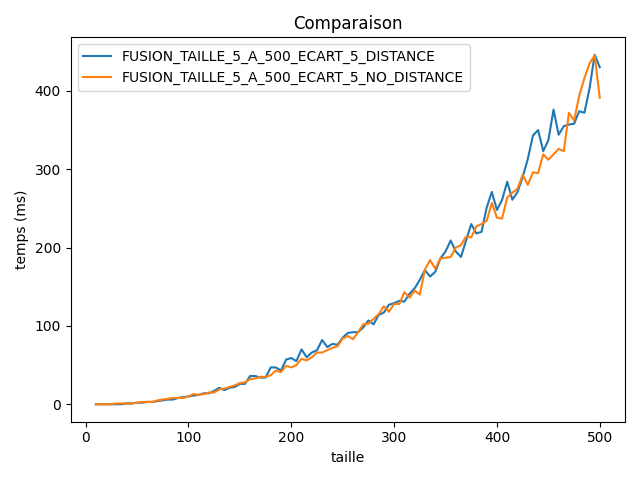
\includegraphics[width=0.8\textwidth]{figures/efficacité/résultats/labyrinthes_parfaits/fig_4.png}
    \caption{$a = \text{FUSION}, n = 5, e = 5, f = 500$}
    \label{fig:efficacité_résultats_4}
\end{figure}

\begin{figure}[H]
    \centering

    %===========================
    %  FUSION — Distance
    %===========================
    \begin{subfigure}{0.45\textwidth}
        \centering
        \begin{tabular}{|r|r|}
            \hline
            Taille & Temps (ms) \\
            \hline
            10  & 0 \\
            50  & 2 \\
            100 & 10 \\
            150 & 26 \\
            200 & 59 \\
            250 & 85 \\
            300 & 129 \\
            350 & 195 \\
            400 & 248 \\
            450 & 337 \\
            500 & 430 \\
            \hline
        \end{tabular}
        \caption{FUSION — Distance}
    \end{subfigure}
    \hfill
    %===========================
    %  FUSION — Sans distance
    %===========================
    \begin{subfigure}{0.45\textwidth}
        \centering
        \begin{tabular}{|r|r|}
            \hline
            Taille & Temps (ms) \\
            \hline
            10  & 0 \\
            50  & 2 \\
            100 & 10 \\
            150 & 27 \\
            200 & 47 \\
            250 & 84 \\
            300 & 128 \\
            350 & 187 \\
            400 & 238 \\
            450 & 312 \\
            500 & 391 \\
            \hline
        \end{tabular}
        \caption{FUSION — Sans distance}
    \end{subfigure}

    \caption{Résultats FUSION pour les tailles 10–500}
\end{figure}

\newpage

\subsubsection{Comparaisons inter-algorithmes}

\textbf{Parfaits / Fusion}

\begin{figure}[H]
    \centering
    
\includegraphics[width=0.8\textwidth]{figures/efficacité/résultats/comparaisons_inter-algorithmes/fig_1.png}
    \caption{Comparaison des performances entre PERFECT et FUSION}
    \label{fig:efficacité_résultats_1}
\end{figure}

\obs{L'algorithme par fusion est sans surprise moins performant, mais les performances restent largement acceptables pour les tailles testées.}

\newpage
\textbf{Parfaits / Aléatoires}

\begin{figure}[H]
    \centering
    
\includegraphics[width=0.8\textwidth]{figures/efficacité/résultats/comparaison_parfaits__aléatoires/fig_1.png}
    \caption{Comparaison PERFECT (TP) / RANDOM}
    \label{fig:efficacité_résultats_2}
\end{figure}

\obs{Comme prévu, les labyrinthes ont une efficacité très proche, la seule différence notable étant conceptuelle (distance entrée/sortie maximale imposée pour la courbe RANDOM\_DISTANCE).}

\newpage

\subsection{Conclusion}

Dans tous nos algorithmes, la représentation du labyrinthe repose sur la même structure que dans le TP2 : deux tableaux de booléens pour les murs horizontaux et verticaux. La comparaison des performances se fait donc à structure de données identique, par conséquent les écarts observés proviennent uniquement des algorithmes de génération eux-mêmes.

Sur la plage de tailles testées (de $10 \times 20$ à $500 \times 1000$), l’algorithme \texttt{PERFECT} issu du TP2 (parcours en profondeur) est systématiquement plus rapide que l’algorithme par fusion. Pour les grandes tailles, on observe qu’un labyrinthe généré par \texttt{PERFECT} est de l’ordre de dix fois plus rapide à produire qu’avec l’algorithme de fusion intégrant le calcul de distance.

Cette différence s’explique par les structures auxiliaires utilisées : \texttt{PERFECT} ne s’appuie que sur une pile de positions et un tableau de booléens \texttt{visited}, alors que l’algorithme de fusion maintient en plus des tableaux \texttt{parent[]} et \texttt{size[]} pour la structure Union--Find et effectue davantage de tirages aléatoires.

Du point de vue de la représentation du labyrinthe, nous en concluons que la structure héritée du TP2 (deux tableaux de booléens) est suffisamment efficace et ne constitue pas un goulot d'étranglement : le coût principal vient de la logique de génération. L'algorithme \texttt{PERFECT} est donc à privilégier lorsque la performance est prioritaire, tandis que l'algorithme de fusion, plus coûteux, se justifie surtout pour des raisons esthétiques, les labyrinthes obtenus étant généralement jugés plus « visuels », bien qu'ils restent, dans les deux cas, parfaitement parfaits.

\newpage

\section{Complément et Bilan}

\subsection{Complément}

\subsubsection{Algorithme de fusion}

Comme indiqué dans la section \textbf{Algorithmes de génération}, des efforts d'optimisation ont été réalisés sur l'algorithme de fusion. Nous présentons ici la comparaison de performances ayant motivé ces changements.

\begin{figure}[H]
    \centering
    
\includegraphics[width=0.8\textwidth]{figures/complément_et_bilan/complément/algorithme_de_fusion/fig_1.png}
    \caption{Performances de la version initiale avant optimisation}
    \label{fig:complément_et_bilan_complément_1}
\end{figure}

\subsubsection{Distance entrée/sortie}

Notre solution actuelle est optimisée, mais elle n'est apparue qu'après plusieurs tentatives. En effet, notre première solution consistait à :

\begin{itemize}
\item Faire un dictionnaire (clé : Position, valeur : Distance) de toutes les positions depuis la position de départ par parcours en largeur.
\item Puis, choisir toutes les positions satisfaisant la distance cible parmi toutes celles explorées.
\end{itemize}

En réalité, cette approche est inefficace puisqu'elle implique de parcourir absolument tout le labyrinthe, même quand la distance cible est petite. Elle avait été retenue comme solution simple au problème de la détermination de la distance maximale possible.

\textbf{Optimisation : Arrêt anticipé par niveaux}

La solution optimisée exploite la nature par niveaux du parcours en largeur :
\begin{itemize}
    \item On traite le parcours en largeur niveau par niveau (toutes les positions à distance $d$) au lieu de position par position.
    \item Dès qu'on atteint le niveau cible, on récupère toutes les positions de ce niveau et on s'arrête immédiatement.
    \item Si la distance cible dépasse la distance maximale du labyrinthe, on retourne les positions du dernier niveau atteint.
\end{itemize}

Cette optimisation évite d'explorer inutilement tout le labyrinthe. Pour les labyrinthes parfaits avec une distance entrée/sortie modérée, le gain est considérable.

Les performances de l'algorithme parfait ont été multipliées par 10 après application de cette nouvelle solution.

Classe : \href{https://gitlab.univ-lille.fr/sae302/2025/G2_SAE3.3/-/blob/master/labyrinth/src/main/java/fr/univlille/labyrinth/model/algorithm/pathsearch/MazeDistance.java?ref_type=heads}{\texttt{MazeDistance.java}}

\newpage

\textbf{Les sous-sous-sections suivantes ne portent plus sur la génération de labyrinthes. Elles présentent l’implémentation d’algorithmes, proches de ceux utilisés précédemment mais appliqués à d’autres tâches, afin d’illustrer l’extensibilité et la réutilisabilité de notre approche algorithmique.}

\subsubsection{Placement des entités}

Notre projet comporte des \textbf{entités} (\emph{joueurs, monstres, sorties...}) qui doivent être placées initialement selon des stratégies. Le problème étant très similaire à celui du placement de l'entrée et de la sortie, un algorithme de la sorte a été implémenté pour le calcul de leurs positions de départ.

La différence étant que le placement vérifie l'absence d'entités sur cette case. L'algorithme enlève alors les positions occupées pour le niveau exploré. Si le niveau demandé ne comporte aucune position valide, alors nous explorons un niveau supérieur.

Classes concernées :
\begin{itemize}
    \item \texttt{fr.univlille.labyrinth.model.maze.entities.PlayerEntity} : méthode \texttt{getInitialPosition(ObservableMaze)}
    \item \texttt{fr.univlille.labyrinth.model.maze.entities.MonsterEntity} : méthode \texttt{getInitialPosition(ObservableMaze)}
    \item \texttt{fr.univlille.labyrinth.model.maze.entities.ExitEntity} : méthode \texttt{getInitialPosition(ObservableMaze)}
    \item \texttt{fr.univlille.labyrinth.model.maze.entities.factory.EntityListFactory} : méthode \texttt{fillMazeEntities(ObservableMaze, String)}
\end{itemize}

\href{https://gitlab.univ-lille.fr/sae302/2025/G2_SAE3.3/-/tree/master/labyrinth/src/main/java/fr/univlille/labyrinth/model/maze/entities}{Package \texttt{entities}}


\subsubsection{Déplacement des monstres}

Notre projet comporte des \textbf{monstres}, entités qui cherchent à toucher le joueur pour mettre fin à sa partie.

Le monstre se déplace en fonction du meilleur chemin vers le joueur, donné par une fonction implémentant un parcours en largeur. Le monstre choisit donc toujours le chemin optimal vers le joueur.

Classes concernées :
\begin{itemize}
    \item \texttt{fr.univlille.labyrinth.model.maze.entities.movebehaviors.MonsterMoveBehavior} : méthode \texttt{move(Entity, Direction, ObservableMaze)}
    \item \texttt{fr.univlille.labyrinth.model.algorithm.pathsearch.MazePath} : méthode \texttt{pathFinder(Maze, Position, Position)}
\end{itemize}

\newpage

\subsection{Bilan}

\subsubsection{Difficultés}

Les principales difficultés rencontrées lors du développement de la partie algorithmique incluent :

\begin{enumerate}
    \item \textbf{Compréhension de l'Union-Find} : La structure de données Union-Find avec ses optimisations (compression de chemin et union par taille) n'est pas intuitive. Il a fallu étudier l'algorithme de Kruskal et comprendre comment adapter cette structure au problème de génération de labyrinthe.

    \item \textbf{Gestion de la distance entrée/sortie} : Gérer le cas où la distance demandée dépasse la distance maximale possible dans le labyrinthe a nécessité une conception soignée de l'algorithme de parcours en largeur avec arrêt anticipé.

    \item \textbf{Placement des entités} : Adapter l'algorithme de distance pour placer plusieurs entités (joueurs, monstres) sans collision tout en respectant les contraintes de distance a demandé de la réflexion et des tests pratiques.
\end{enumerate}

\subsubsection{Limites}

Malgré les optimisations apportées, certaines limites subsistent :

\begin{enumerate}
    \item \textbf{Labyrinthes aléatoires avec distance maximale} : Pour les labyrinthes aléatoires, la distance entrée/sortie est imposée au maximum possible par le sujet. Cela force l'algorithme de distance à explorer tout le labyrinthe, ce qui devient coûteux pour de très grandes tailles (voir benchmarks : 214 ms pour $500 \times 1000$ avec distance contre 54 ms sans).

    \item \textbf{Variance des performances} : Les temps de génération varient selon l'aléatoire. Pour un labyrinthe $500 \times 1000$ avec fusion, on observe des variations de $\pm 10\%$ entre différentes exécutions. C'est pourquoi nos benchmarks calculent une moyenne sur plusieurs exécutions.
\end{enumerate}

\subsubsection{Améliorations}

Plusieurs axes d'amélioration pourraient être explorés :

\begin{enumerate}
    \item \textbf{Parallélisation} : La génération de plusieurs labyrinthes pourrait être parallélisée. Cela serait utile pour l'application si on souhaite générer plusieurs niveaux à l'avance.

    \item \textbf{Cache de labyrinthes} : Pré-générer et mettre en cache des labyrinthes de tailles courantes pour accélérer le démarrage de parties. Les labyrinthes parfaits étant déterministes (modulo l'aléatoire), on pourrait stocker des graines aléatoires intéressantes.

    \item \textbf{Génération progressive} : Pour de très grands labyrinthes, générer par régions au fur et à mesure que le joueur explore, plutôt que tout d'un coup. Cela permettrait des labyrinthes théoriquement illimités.

    \item \textbf{Optimisation de la distance pour labyrinthes aléatoires} : Actuellement, on explore tout le labyrinthe pour trouver la distance maximale. On pourrait estimer cette distance de manière heuristique (par exemple, distance Manhattan $\times$ facteur de correction) pour éviter l'exploration complète.

    \item \textbf{Algorithmes de génération alternatifs} : Implémenter d'autres algorithmes classiques (Prim, Eller, récursive division) pour offrir plus de variété visuelle dans les labyrinthes générés.

    \item \textbf{Métriques de qualité} : Développer des métriques pour évaluer la "qualité" d'un labyrinthe (nombre de culs-de-sac, longueur moyenne des couloirs, etc.) et permettre de régénérer si un labyrinthe ne répond pas aux critères.
\end{enumerate}

\section{Conclusion}

La solution présentée répond pleinement aux exigences du jalon 2 et établit des bases solides et durables pour l’algorithme de génération de labyrinthes.

\end{document}






